\documentclass[xcolor=dvipsnames, USenglish]{beamer}  %notes=show to print them in the generated pdf
% Packages for a reasonable beamer session
\usepackage[T1]{fontenc}
%\usepackage[ansinew]{inputenc}
\usepackage[utf8]{inputenc}
\usepackage{textcomp}
\usepackage{lmodern}
\usepackage{csquotes}
\usepackage[english]{babel}
%\usepackage{babel}

\usepackage{graphicx}

\usepackage{amsmath}
\usepackage{amsfonts}
\usepackage{amssymb}
\usepackage{amsthm}
\usepackage{bm}

\usepackage{booktabs}
\usepackage{tabularx}

\usepackage{hyperref}

\usepackage{ellipsis}

% Additional packages
\usepackage{graphicx}
\usepackage{subfigure}
\usepackage{xcolor}
\usepackage{minted}

\usepackage[style=authoryear, backend=biber]{biblatex}
\setbeamertemplate{itemize/enumerate body begin}{\setlength{\leftmargini}{1.5em}}
\renewcommand*{\nameyeardelim}{\addcomma\addspace}
\addbibresource{\jobname.bib}
\renewcommand{\footnotesize}{\tiny}

\usepackage{tikz,pgf,calc}
%\usetikzlibrary{matrix, shapes, positioning, calc,
%  decorations.pathreplacing, shapes.geometric, arrows}
\usetikzlibrary{shapes.geometric, arrows, calc}
\tikzstyle{startstop} = [rectangle, rounded corners, minimum width=3cm, minimum height=1cm, text centered, text width=1.5cm, draw=black, fill=red!30]
\tikzstyle{io} = [trapezium, trapezium left angle=70, trapezium right angle=110, minimum width=3cm, minimum height=1cm, text centered, draw=black, fill=blue!30]
\tikzstyle{process} = [rectangle, minimum width=3cm, minimum height=1cm, text centered, draw=black, fill=orange!30]
\tikzstyle{decision} = [diamond, minimum width=3cm, minimum height=0.5cm, text centered, draw=black, fill=green!30]
\tikzstyle{arrow} = [thick,->,>=stealth]

%% References
\newlength\leftsidebar
\makeatletter
\setlength\leftsidebar{\beamer@leftsidebar}
\makeatother

\usepackage[absolute,overlay]{textpos}
\newenvironment{reference}[2]{%
  \begin{textblock*}{\textwidth}(\leftsidebar+#1,\paperheight-#2)
      \scriptsize\bgroup\color{red!50!black}}{\egroup\end{textblock*}}

% Path to graphics
\graphicspath{{../img/}}

% Sources
\usepackage{setspace}
\newcommand{\source}[1]{\begin{spacing}{0.5}{\fontsize{5}{6}\selectfont source: \itshape {#1}}\end{spacing}}
 % PACKAGES
% Collection of useful mathematical symbols and commands
% Calculus
\newcommand{\ud}{\mathrm{d}}
\newcommand{\pder}[2]{\frac{\partial{#1}}{\partial{#2}}}
\newcommand{\dpder}[2]{\frac{\partial^2{#1}}{\partial{#2^2}}}
\newcommand{\sderp}[3]{\frac{\partial^2{#1}}{\partial{#2}\partial{#3}}}
\newcommand{\tder}[2]{\frac{\ud{#1}}{\ud{#2}}}
\newcommand{\rot}[1]{\nabla \times {#1}}
\newcommand{\diver}[1]{\nabla \cdot {#1}}
\newcommand{\definter}[4]{\int_{#1}^{#2} {#3}\ud {#4}}
\newcommand{\inter}[2]{\int {#1}\ud {#2}}
\newcommand{\braket}[2]{\langle {#1} , {#2} \rangle}
% Misc
\newcommand{\eval}[1]{\Big |_{#1}}
\newcommand{\bset}[1]{\big\lbrace {#1} \big\rbrace}
\newcommand{\stimes}[2]{{#1}\!\times\!{#2}}
\newcommand{\trp}{\top}
\newcommand{\preup}[2]{{}^{#2}\!{#1}}

% Operators
\DeclareMathOperator*{\armin}{arg\,min}
\DeclareMathOperator*{\armax}{arg\,max}
\DeclareMathOperator*{\rank}{rank}
\DeclareMathOperator*{\cov}{cov}
\DeclareMathOperator*{\nullsp}{null}
% Logicals
\newcommand{\suchthat}{\big \backslash \;}
   % SYMBOLS

% ----------- Extra packages
\usepackage{../beamer_themes/beamerthemeEawag_blue} % Eawag style

% ----------- References used and shown
\begin{filecontents}{\jobname.bib}
@article{Stegenga2011,
author = {Stegenga, Jacob},
doi = {10.1007/s11229-011-9973-x},
journal = {Synthese},
month = {aug},
number = {12},
pages = {2391--2411},
title = {{An impossibility theorem for amalgamating evidence}},
volume = {190},
year = {2013}
}
@online{CPGGreyNormal,
  author = {{CPG Grey}},
  title = {{Quick and Easy Voting for Normal People}},
  year = 2014,
  month= 11,
  url = {https://youtu.be/orybDrUj4vA},
  urldate = {2017-06-16}
}
@online{CPGGreyPolitics,
  author = {{CPG Grey}},
  title = {{Politics in the Animal Kingdom}},
  year = 2014,
  month= 10,
  url = {https://www.youtube.com/playlist?list=PL7679C7ACE93A5638},
  urldate = {2017-06-16}
}
@online{TadashiDice,
  author = {{Numberphile} and Tadashi Tokieda},
  title = {{The Most Powerful Dice}},
  year = 2016,
  month= 09,
  url = {https://youtu.be/zzKGnuvX6IQ},
  urldate = {2017-06-16}
}
\end{filecontents}


% ----------- Extra symbols
\newcommand{\ccov}[1]{{\color{red}k}\left(#1\right)}
\newcommand{\cmean}[1]{{\color{blue}m}\left(#1\right)}
\newcommand{\sm}{\scalebox{0.5}{-1}}

%----------------
% title information
\title{Master Thesis}
\subtitle{Development of an Overland Flow Model Emulator}
\author[\texttt{sebastiano.rusca@eawag.ch}]{Sebastiano Rusca}
\institute[Eawag]{Eawag: Swiss Federal Institute of Aquatic Science
  and Technology}
\date[22.01.2018]{January 22, 2018}

% ====================================================================

\begin{document}

% ----------------
% Title frame
% load background for title
\setbeamertemplate{background}{
  
\includegraphics[width=\paperwidth,height=\paperheight]
  {../beamer_themes/background_title_blue.png}}
{ \setbeamertemplate{footline}{} % no footer on title
  \begin{frame}
    \titlepage
  \end{frame}
}
% load background for all other slides
\setbeamertemplate{background}{

\includegraphics[width=\paperwidth,height=\paperheight]
{../beamer_themes/background_slides_blue.png}}
%\setbeamertemplate{footline}[Sebastiano Rusca] % set footer
\addtocounter{framenumber}{-1}  % don't count title page

%%%%%%%%%%%%%%%%%%%%%%%%%%%%%%%%%%%%%%%%%%%%%%%
% WHAT IS EMULATION
\section{Introduction}

  \begin{frame}
    \frametitle{What is emulation?}
    \begin{itemize}
      \item \textbf{Emulator, aka Surrogate model}: approximation model that mimic
      the behavior of a simulator model as closely as possible\footfullcite{wiki_emulator}
      \begin{itemize}
        \item computationally cheaper to evaluate
        \item constructed with data driven, bottom-up approach
        \item internal states of the simulator model are lost
      \end{itemize}
    \end{itemize}

    \begin{figure}
      \centering
      \begin{subfigure}[b]{0.4\textwidth}
          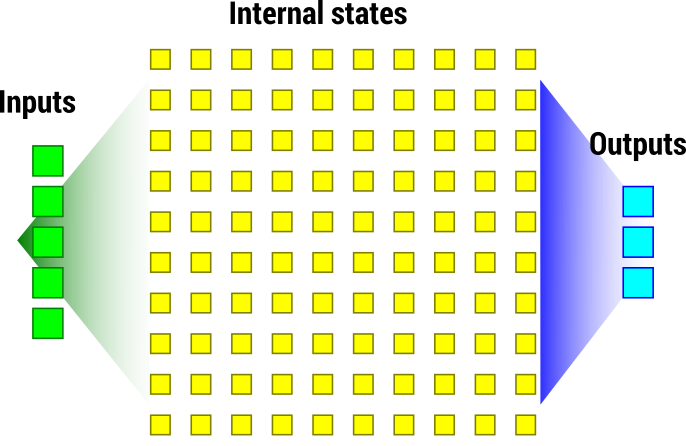
\includegraphics[width=\textwidth]{img/simulator.png}
          \caption{Simulator}
          \label{subfig:simulator}
      \end{subfigure}
      \quad
        %add desired spacing between images, e.g. \quad, \qquad, \hfill etc. 
        %(or a blank line to force the subfigure onto a new line)
      \begin{subfigure}[b]{0.4\textwidth}
        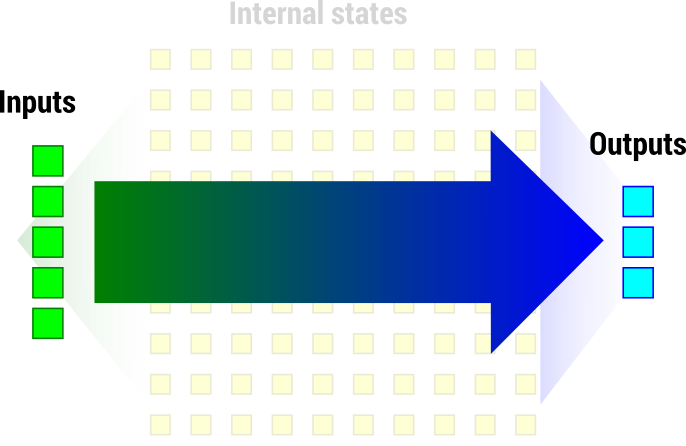
\includegraphics[width=\textwidth]{img/emulator.png}
        \caption{Emulator}
        \label{subfig:emulator}
      \end{subfigure}
    \end{figure}
  \end{frame}

% As you can see from the title my master thesis deals with emulation.
% So first of all let's see what emulation is:
% Emulat

%%%%%%%%%%%%%%%%%%%%%%%%%%%%%%%%%%%%%%%%%%%%%%%%%%%%%%%%%%%%%%%%%%%%%%%%%%%%%%%%
% WHY OVERLAND FLOW

\section{Introduction}
  \begin{frame}
    \frametitle{Why overland flow?}
    \begin{itemize}
      \item very topical issue, also in Switzerland (e.g. flooding in Zofingen)
      \item BAFU and cantons already investigating and taking actions
      \item \textbf{simulators do a good job\ldots but are still too slow}
    \end{itemize}

    \begin{figure}
      \centering
      \begin{subfigure}[b]{0.25\textwidth}
        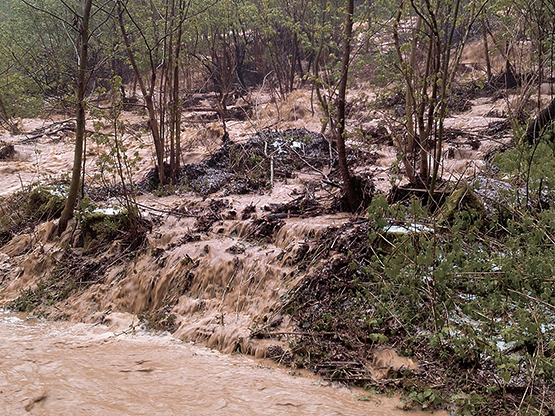
\includegraphics[width=\textwidth]{img/overlandflow1.jpg}
        \label{subfig:ovflow1}
      \end{subfigure}
      \quad
          %add desired spacing between images, e.g. \quad, \qquad, \hfill etc. 
          %(or a blank line to force the subfigure onto a new line)
      \begin{subfigure}[b]{0.25\textwidth}
        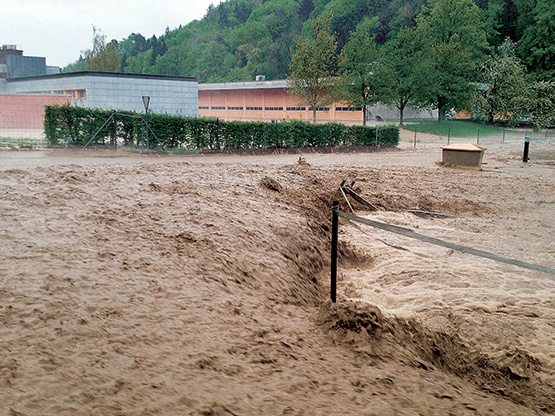
\includegraphics[width=\textwidth]{img/overlandflow2.jpg}
        \label{subfig:ovflow2}
      \end{subfigure}
      
      \begin{subfigure}[b]{0.25\textwidth}
        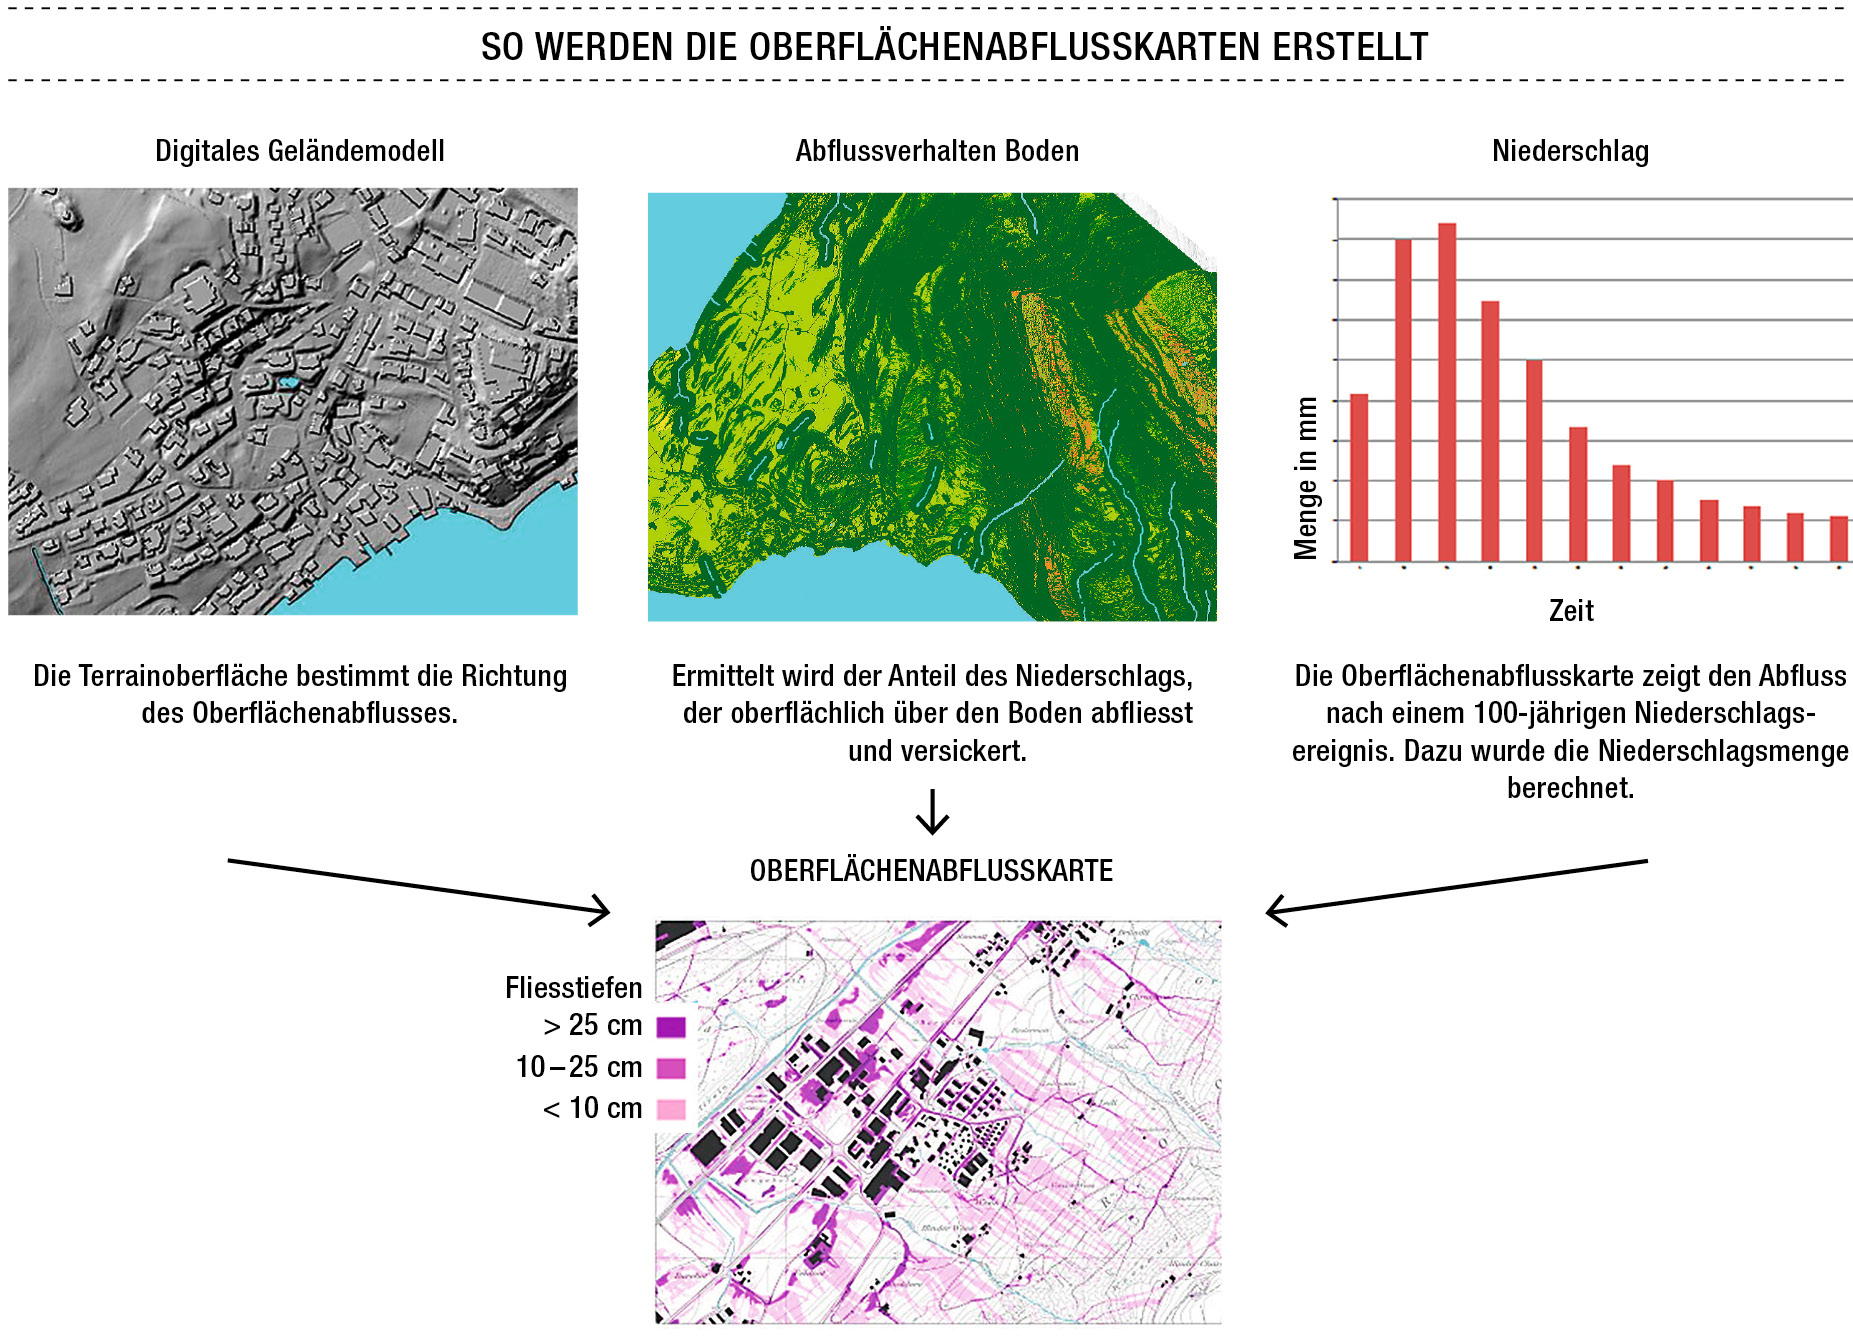
\includegraphics[width=\textwidth]{img/overlandflow_map1.jpg}
        \label{subfig:ovflowmap1}
      \end{subfigure}
      \quad
          %add desired spacing between images, e.g. \quad, \qquad, \hfill etc. 
          %(or a blank line to force the subfigure onto a new line)
      \begin{subfigure}[b]{0.25\textwidth}
        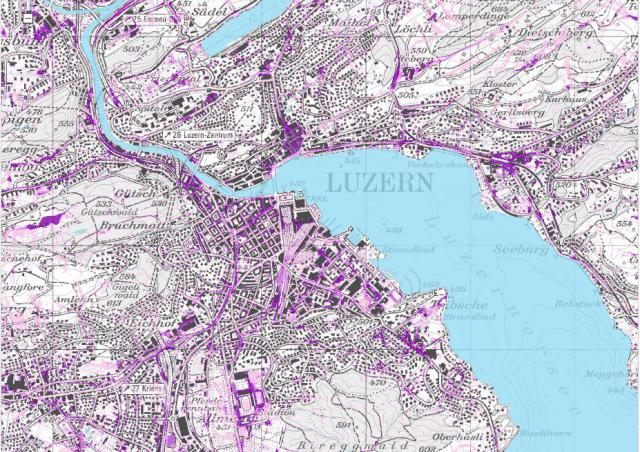
\includegraphics[width=\textwidth]{img/overlandflow_map2.jpg}
        \label{subfig:ovflowmap2}
      \end{subfigure}
    \end{figure}
  \end{frame}

%%%%%%%%%%%%%%%%%%%%%%%%%%%%%%%%%%%%%%%%%%%%%%%%%%%%%%%%%%%%%%%%%%%%%%%%%%%%%%%%
% PROJECT CONCEPT: IDEA

\section{Project concept}
  \begin{frame}
    \frametitle{Project idea}
  \end{frame}

%%%%%%%%%%%%%%%%%%%%%%%%%%%%%%%%%%%%%%%%%%%%%%%%%%%%%%%%%%%%%%%%%%%%%%%%%%%%%%%%
% PROJECT CONCEPT: GOALS

\section{Project concept}
  \begin{frame}
    \frametitle{Project goals}
  
  \end{frame}
  
%%%%%%%%%%%%%%%%%%%%%%%%%%%%%%%%%%%%%%%%%%%%%%%%%%%%%%%%%%%%%%%%%%%%%%%%%%%%%%%%
% FIRST EMULATOR

\section{Project concept}
  \begin{frame}
    \frametitle{First emulation experiment}
  
  \end{frame}
  
%%%%%%%%%%%%%%%%%%%%%%%%%%%%%%%%%%%%%%%%%%%%%%%%%%%%%%%%%%%%%%%%%%%%%%%%%%%%%%%%
% NEXT STEPS

\section{Project concept}
  \begin{frame}
    \frametitle{Next steps}
  
  \end{frame}
\end{document}

